\documentclass[conference, a4paper, final]{IEEEtran} %letterpaper
\usepackage[utf8]{inputenc}
\usepackage{physics}
\usepackage{url}
\usepackage{etoolbox}
\usepackage{nomencl}
\makenomenclature
\makeatletter
\patchcmd{\thenomenclature}{\section*}{\section}{}{}
\makeatother
%\renewcommand{\nomname}{List of Symbols}
%\renewcommand{\nompreamble}{The next list describes several symbols that will be later used within the body of the document}
% This will add the units
%----------------------------------------------
\newcommand{\nomunit}[1]{%
\renewcommand{\nomentryend}{\hspace*{\fill}#1}}
%----------------------------------------------
\usepackage{siunitx}
\usepackage{amssymb}
\usepackage{enumitem}
\usepackage{hyperref}
\renewcommand*{\figureautorefname}{Fig.}




\usepackage{tikz}
\usetikzlibrary{shapes, arrows, calc, positioning, automata}
\tikzstyle{block} = [rectangle, minimum width=1cm, minimum height=1cm, text centered, draw=black, align=center]
\tikzstyle{process} = [rectangle, minimum width=1cm, minimum height=1cm, text centered, draw=black, align=center, text width = 5cm]
\tikzstyle{decision} = [diamond, thick, minimum width=3cm, minimum height=1cm, text centered, draw=black, align=center, text width = 2cm]
\tikzstyle{sum} = [circle, minimum width=1mm, minimum height=1mm, text centered, draw=black, inner sep=0pt]
\tikzstyle{arrow} = [thick,->,>=stealth]
\tikzstyle{startstop} = [rectangle, rounded corners=2.5mm, minimum width=1.5cm, text centered, draw=black]


\title{A novel Implementation Technique for Genetic Algorithm based Auto-Tuning PID Controller
}
\author{\IEEEauthorblockN{Student}
\IEEEauthorblockA{school address}
\and
\IEEEauthorblockN{Antonio}
\IEEEauthorblockA{UAC address}
\and
\IEEEauthorblockN{Co-Author}
\IEEEauthorblockA{UAC address}
\and
\IEEEauthorblockN{S. K. Gadi}
\IEEEauthorblockA{FIME, Universidad Autónoma de Coahuila,\\
Torreón, Coahuila, México.\\
Tel.: (+52 1) 871 757 0239\\
Fax: (+52 1) 871 757 0239\\
Email: research@skgadi.com}}

\hyphenation{op-tical net-works semi-conduc-tor}

\begin{document}
\maketitle

\begin{abstract}
The auto-tuning proportional-integral-derivative (PID) controllers based on genetic algorithms have many limitations in its implementation. This article presents such limitations and provides the possible solutions. An implementation technique is proposed based on these solutions. Numerical simulations are given to evaluate the proposed method applied to a system with variable parameters, a non-linear system and a time delayed system. This technique is used to control a DC servo motor. These results coincide with the obtained simulation results.
\end{abstract}
\IEEEpeerreviewmaketitle
\section{Introduction}
Theoretically, a proportional-integral-derivative (PID) controller guarantees stability for lower order linear systems [Please correct and provide citation]. However, these are used in many industries to control nonlinear and delayed systems \cite{ang2005pid, o2003pid}. A nonlinear system behaves like a linear system under certain operating conditions. Hence stability is achieved by a PID controller for a particular operating condition. The PID parameters must be updated when the operating conditions change for a stable operation. In the case of a delayed system, apart from the PID parameters the transportation delay also plays a significant role in its stability. In some cases, introducing an additional delay into the system stabilizes a system.
%Nomenclature
\printnomenclature

\section{PID controller}
\begin{figure}
\centering
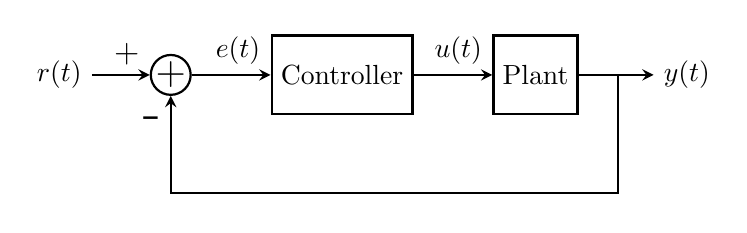
\begin{tikzpicture}[auto, thick, node distance=1cm, >=triangle 45]
    \node (Sum0) [sum] {\Large $+$};
    \node (Control) [block, right = of Sum0] {Controller};
    \node (Plant) [block, right = of Control] {Plant};
    \coordinate[right of = Plant, node distance=1.5cm] (End);
    \coordinate[left of = Sum0, node distance=1cm] (Start);
    \draw [arrow] (Start)[anchor= east] node{$r(t)$} -- (Sum0) node [pos=1.0, anchor = south east]{\large +};
    \draw [arrow] (Sum0) -- (Control) node [pos=1.0, anchor = south east ]{$e(t)$};
    \draw [arrow] (Control) -- (Plant) node [pos=1.0, anchor = south east ]{$u(t)$};
    \draw [arrow] (Plant) -- (End) node [pos=1.0, anchor = west ]{$y(t)$};
    \draw [arrow] ($(Plant.east) + (5mm,0mm)$) |- node[pos=0.75, inner sep=2pt]{}++(-1,-1.5) -| (Sum0.south) node[anchor=north east]{\huge -};
\end{tikzpicture}
\caption{Closed loop system}
\label{Fig:ClosedLoopSystem}
\end{figure}
\autoref{Fig:ClosedLoopSystem} shows a typical closed loop system with negative feedback. The plant and controller blocks represent its dynamics. $r(t)$, $u(t)$, $y(t)$ and $e(t) = r(t)-y(t)$ are reference, control, output and error signals respectively. The objective of a controller is to achieve $$\lim_{t\rightarrow \infty}{e(t)} = 0.$$
\nomenclature{$r$}{Reference signal}
\nomenclature{$u$}{Control signal}
\nomenclature{$y$}{Output of the plant}
\nomenclature{$e$}{Error between reference and measured plant output}
\nomenclature{$t$}{Time}%\nomunit{\si{\second}}}

\par
A PID controller is defined as
\begin{eqnarray}
    u(t) &=& K_Pe(t) + K_I\int{e(t)\dd{t}} + K_D\dv{t}(e(t)), \label{Eqn:PIDDefinition}
\end{eqnarray}
where $K_P$, $K_I$, and $K_D$ are nonnegative constant values. These parameters are tuned to achieve stability.
\nomenclature{$K_P$}{Proportional constant of PID controller}
\nomenclature{$K_I$}{Integral constant of PID controller}
\nomenclature{$K_D$}{Derivative constant of PID controller}
\par
Usually, sensors are used to measure the output of the plant $y(t)$ which are prone to noise. The noise power is amplified when differentiation is performed \cite{mathworks2017}. Therefore instead of using the PID controller as it is the third term associated with the derivative is modified as a filter. Modified version of PID controller in frequency domain is
\begin{eqnarray}
    u(s) &=& K_Pe(s) + \frac{K_Ie(s)}{s} + \frac{K_De(s)s}{s+N}, \label{Eqn:ModifiedPIDDefinition}
\end{eqnarray}
where $s$ is the Laplace transform's complex variable and $N>>1$ is a constant.
\nomenclature{$s$}{Laplace transform's complex variable}
\nomenclature{$N$}{Constant associated with the filter implementing the derivative term in a PID controller}
\par
Tuning a PID controller is a task of selecting optimal values for the four parameters $K_P$, $K_I$, $K_D$, and $N$ for which the plant is stable with required performance. The required performance can be ensuring settling time, providing damping or improving raise time, etc. In practice, $N$ is kept constant. However, in this article $N$ is considered as one of the tunable parameters.
\par
The next section presents a typical method for tuning these parameters with the help of a genetic algorithm.
\section{Conventional Genetic Algorithm based PID tuning}
\begin{figure}
\centering
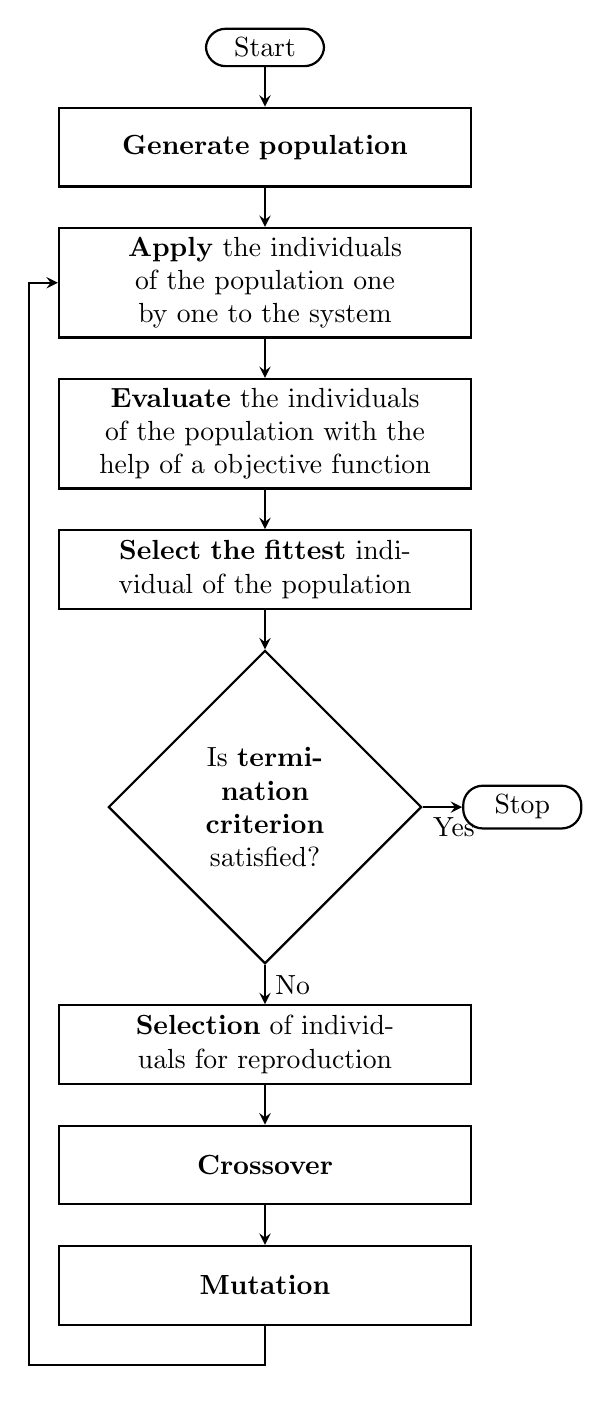
\begin{tikzpicture}[auto, thick, node distance=5mm, >=triangle 45]
    \node (Start) [startstop] {Start};
    \node (CreatePopulation) [process, below = of Start] {\textbf{Generate population}};
    \node (ApplyPopulation) [process, below = of CreatePopulation] {\textbf{Apply} the individuals of the population one by one to the system};
    \node (EvaluatePopulation) [process, below = of ApplyPopulation] {\textbf{Evaluate} the individuals of the population with the help of a objective function};
    \node (SelectFittest) [process, below = of EvaluatePopulation] {\textbf{Select the fittest} individual of the population};
    \node (DecideToStop) [decision, below = of SelectFittest] {Is \textbf{termination criterion} satisfied?};
    \node (Selection)  [process, below = of DecideToStop] {\textbf{Selection} of individuals for reproduction};
    \node (Crossover)  [process, below = of Selection] {\textbf{Crossover}};
    \node (Mutation)  [process, below = of Crossover] {\textbf{Mutation}};
    \node (Stop) [startstop, right = of DecideToStop] {Stop};
    \draw [arrow] (Start) -- (CreatePopulation);
    \draw [arrow] (CreatePopulation) -- (ApplyPopulation);
    \draw [arrow] (ApplyPopulation) -- (EvaluatePopulation);
    \draw [arrow] (EvaluatePopulation) -- (SelectFittest);
    \draw [arrow] (SelectFittest) -- (DecideToStop);
    \draw [arrow] (DecideToStop.south) node[anchor=north west]{No} -- (Selection);
    \draw [arrow] (DecideToStop.east) node[anchor=north west]{Yes} -- (Stop);
    \draw [arrow] (Selection) -- (Crossover);
    \draw [arrow] (Crossover) -- (Mutation);
    \draw [arrow] (Mutation.south) |- node[pos=0.75, inner sep=2pt]{}++(-3,-0.5) |- (ApplyPopulation.west);
\end{tikzpicture}
\caption{Conventional genetic algorithm based PID tuning algorithm}
\label{Fig:ConventionalGAPIDTuning}
\end{figure}
\autoref{Fig:ConventionalGAPIDTuning} shows a standard genetic algorithm based PID tuning algorithm \cite{kim2008auto, ZEMMIT2017}. In this context, the word population is used to represent a fixed set of individuals or chromosomes; and an individual or a chromosome represents an array of values for the parameters to be tuned. In this case the parameters are $K_P$, $K_I$, $K_D$ and $N$. Each chromosome is a candidate for the optimal solution. The genetic algorithm mimics the evolution process to generate optimal values for the parameters. It starts with a generation of a random population; it undergoes reproduction and mutation process to produce a next generation population with values much closer to the optimal values. This algorithm includes the following operations.
\begin{description}
    \item[Generate population:] A predetermined number of random chromosomes, $C\in \mathbb{R}^{n\times 4}$, are created to group them as a first generation population. The constant $n$ represents the population size. The random numbers are scaled to match the upper and lower limits of the parameters. In this case, the random numbers must be greater than zero.
    \item[Apply:] The values for the tunable parameters of the closed-loop system, $K_P$, $K_I$, $K_D$ and $N$ are replaced by each of the present generation's chromosomes, $C_i\mathbb{R}^{4}$, one after another for the time-period $[T_{i^-}, T_{i^+})$. This process repeats $n$ times. Here $C_i$, $i \in \{1, 2, 3, \dots, n\}$ represents the $i$\textsuperscript{th} chromosome of the population, $T_{i^-}$ and $T_{i^+}$ start and end time of the implementation of the $i$\textsuperscript{th} chromosome. Since one chromosome is applied after another $T_{i^+} = T_{i+1^-}$.
    \item[Evaluate:] The objective function or the cost function determines how suitable is a chromosome for the closed-loop system. The scale ranges from 0 to $\infty$, where zero associated with the optimal value. In the literature, a variety of cost functions such as mean square error (MSE), integration of time multiplied by absolute error (ITAE), integral of the absolute magnitude of the error (IAE),  integral of the squared error (ISE) and root mean square error (RMSE) are utilized \cite{1300705, kim2008auto}. In this article, the objective function uses RMSE defined as $$RMSE = \frac{1}{T}\int_{T_{i^-}}^{T_{i^+}} \sqrt{(e(t))^2} \dd t,$$ where $T = T_{i^+}-T_{i^-}$ is the time interval for which the $i$\textsuperscript{th} chromosome is applied.
    \item[Select the fittest:] The fittest chromosome in the present generation of the population is the one which produced minimum value for the cost function.
    \item[Termination criterion:] In the practical implementation, the objective function never reaches to a zero value. Hence, the chromosome which offers the objective function below a certain predetermined value is considered optimal. If all of the chromosomes fail to provide optimal results, a new generation is created and evaluated.
    \item[Selection:] This is the first stage of the reproduction process. In this juncture, some chromosomes from the present population are selected to involve in the reproduction process. Roulette wheel selection, stochastic universal sampling,  normalized geometric selection, and tournament selection are the most commonly used selection process methods \cite{gen2000genetic, kim2008auto}. This article uses roulette wheel selection method.
    \item[Crossover:] This is another stage of the reproduction process, where the selected chromosomes undergo the crossing. It is carried out by 1) splitting the selected or parent chromosomes array at a random point and then 2.) the children chromosomes form by joining one parent's front end of separated array with the rear end of another.
    \item[Mutation:] In this stage of the reproduction process, at randomly locations the values are changed. The mutation rate determines the number of mutations. Usually, it is less than 1\%.
\end{description}
\nomenclature{$C$}{Population\nomunit{$\mathbb{R}^{n\times 4}$}}
\nomenclature{$n$}{Population size}
\nomenclature{$C_i$}{$i$\textsuperscript{th} chromosome of the population\nomunit{$\mathbb{R}^{4}$}}
\nomenclature{$T_{i^-}$}{Start time of the implementation of the $i$\textsuperscript{th} chromosome}
\nomenclature{$T_{i^+}$}{End time of the implementation of the $i$\textsuperscript{th} chromosome}
\nomenclature{$T$}{Time interval for which the $i$\textsuperscript{th} chromosome is applied}
\nomenclature{}{}
Since this algorithm uses random values for many of its operations, the optimum values may vary every time we restart the process. The next section presents the problems associated with the implementation of this algorithm.
\section{Problems in the implementation}
\section{Proposed algorithm}
\section{Simulation results}
\section{Experimental results}
\section{Conclusions}
\bibliographystyle{IEEEtran}
\bibliography{refs}
\end{document}


